% !TeX spellcheck = sk_SK-Slovak
\chapter{Zovšeobecnenie sofvéru}

Obsahom tejto kapitole sú úpravy a vylepšenia softvéru tak aby bol jednoduchší na používanie pre používateľa a aby ho bolo možné jednoducho modifikovať pre získavanie dát zo správ pacientov s iným ochorením ako je COVID-19 respektíve pre iných informácii nachádzajúcich sa každej prepúšťacej správe.  

\section{Oddelenie hľadaných informácii od funkcii na hľadanie}

Náš systém mal pôvodne výzor skriptu napísaného v programovacom jazyku Python ktorý obsahoval všetky informácie o tom aká informácie hľadáme a pre nich špecifické regulárne výrazy a aj funkcie ktoré ich dáta pomocou nich a všeobecnejších regulárnych výrazov získavali. Tento prístup je však neprakticky z pohľadu užívateľa keďže ak by chcel upraviť aké dáta sa získavajú musí pracovať priamo so skriptom. Preto sme sa rozhodli informácia ktoré dáta chceme extrahovať a ako by mali byť zapísané v správe do samostatného súbor. Pre čo najlepšiu čitateľnosť súboru používateľom sme si pre tento účel vybrali formát YAML. Ide o človekom ľahko čitateľný súborový formát určený na serializáciu dát \cite{YAML}, vďaka čomu je perfektný pre naše použitie. 

\section{Obsah YAML súboru}

Obsah súboru ''informations.yml'' môžeme rozdeliť do niekoľko častí. Prvou časťou je čast ''vyberove'' v tejto časti je niekoľko riadkov obsahujúcich názov informácia a boolean (pravda/nepravda) hodnotu ktorými hovoríme nášmu systému či má danú informáciu zo správy získavať konkrétne ide o informácie z hlavičky správy, veku, doby hospitalizácie, výške a váhe, saturácii kyslíka v krvi, oxygenoterapii, hospitalizácii na jednotke intenzívnej starostlivosti a smrti pacienta. Takmer všetky tieto hodnoty sú vzájomne nezávislé avšak výnimkou sú vek pacienta a doba hospitalizácie ktoré je možné získavať iba ak je získavaná informácia z hlavičky preto v prípade hodnoty false pre hlavičku sa tieto informácie nebudú získavať bez ohľadu na ich hodnotu.
Druhá časť s názvom ''lieky'' obsahuje lieky o ktorých chceme vedieť či ich pacient užíval. Jednotlivé lieky sú v zaznamenávané následovne, ako prvé jeden názov stĺpca do ktorého sa bude zapisovať informácia či pacient užíval daný liek (väčšinou je to názov samotného lieku) následne je napísaná dvojbodka za ktorú sa nachádza zoznam najbežnejších názvov lieku (zoznam je ohraničený hranatými zátvorkami, jednotlivé názvy sú v apostrofoch a sú oddelené čiarkami) pričom všetky písmená v týchto názvoch musia byť malé keďže náš systém získava túto informáciu z textu ktorý si upravuje tak aby aby boli všetky písmená malé. Na obrázku \ref{obr:lieky_yaml} vidíme ukážku pre liek kolchicín. 
V tretej časti s názvom ''choroby'' sú choroby pri ktorých chceme zistiť či nimi náš pacient netrpí respektíve či ich neprekonal, z pohľadu spôsobu zápisu je táto časť totožná s časťou ''lieky'', malým rozdielom je, že sa tu pre danú chorobu zväčša nachádza viac spôsobov zápisu keďže jedna choroba môže mať viacero označení a skratiek zároveň sú tieto názvy často aj viacslovné a môžu byť rôzne vyskloňované preto si občas vyžadujú  mierne komplikovanejšie regulárne výrazy na ich hľadanie. Takisto aj v prípade skratiek treba zaručiť aby nájdená skratka nebola iba podskraktou inej skratky respektíve náhodnou súčasťou textu napísaného výlučne veľkými písmenami. Na obrázku \ref{obr:choroby_yaml} vidíme ukážku zápisu pre srdcové zlyhávanie.
Vo štvrtej časti nazvanej ''vysledky'' sa nachádzajú informácie ktorých hodnoty chceme získať z krvných testov ktoré boli pacientovi vykonané. Štruktúra zápise je zase totožne s častou ''lieky'' bez významných špecifík. 
Posledná a asi najkomplikovanejšia časť má názov ''protilatky'' táto časť je určená na špecifikáciu choroby respektíve patogénu a názvov protilátok pre získavanie výsledkov testov na tieto protilátky. Každý takto získavaný výsledok sa do súboru zapisuje následovne, do prvého riadku zapíšeme názov, tento názov je pre náš systém irelevantný a slúži iba ako označenie aby používateľ vedel určiť aký test je hľadaný, nasledujú tri riadky ktoré sú odsadené tabulátorom a majú pevne stanovené názov a štruktúru. Prvý z týchto riadkov s názvom ''nazvy\_stlpcov'' obsahuje zoznam názvov stĺpcov pre jednotlivé získavané protilátky, druhý sú ''nazvy\_ochorenia'' to je zoznam názvov pre ochorenie respektíve patogén na ktorého skúmame prítomnosť protilátok u pacienta a v treťom riadku s názvom ''nazvy\_protilatok'' sa nachádza zoznam názvov protilátok ktoré skúmame, pre druhý a tretí riadok platí, že názvy musia obsahovať iba malé písmená. V prípade, že zoznam ''nazvy\_protilatok'' je neprázdny jeho dĺžka (počet záznamov v ňom) musí byť totožná s dĺžkou zoznamu ''nazvy\_stlpcov''. Špeciálny prípad je ak zoznam ''nazvy\_protilatok'' je prázdny v takomto prípade systém nebude pre dané ochorenie hľadať výsledky testov na protilátky proti danému patogénu ale bude hľadať výsledky testov na prítomnosť daného patogénu respektíve testov na dané ochorenie. Konkrétnu ukážku zápisu pre vírus SARS-CoV-2 vidíme na obrázku \ref{obr:protilatky_yaml}.

\begin{figure}
	%vlozenie samotneho obrazku vycentrovaneho a vhodnej velkosti
	%obrazok je v subore images/cervik.png
	\centerline{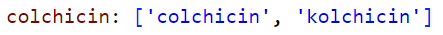
\includegraphics[width=0.5\textwidth]{images/lieky_yaml}}
	%popis obrazku
	\caption[Ukážka zápisu lieku]{Ukážka zápisu skúmaného lieku do YAML súboru}
	%id obrazku, pomocou ktoreho sa budeme na obrazok odvolavat
	\label{obr:lieky_yaml}
\end{figure}

\begin{figure}
	%vlozenie samotneho obrazku vycentrovaneho a vhodnej velkosti
	%obrazok je v subore images/cervik.png
	\centerline{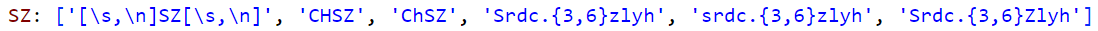
\includegraphics[width=1.05\textwidth]{images/choroby_yaml}}
	%popis obrazku
	\caption[Ukážka zápisu choroby]{Ukážka zápisu skúmaného choroby do YAML súboru}
	%id obrazku, pomocou ktoreho sa budeme na obrazok odvolavat
	\label{obr:choroby_yaml}
\end{figure}
  
\begin{figure}
	%vlozenie samotneho obrazku vycentrovaneho a vhodnej velkosti
	%obrazok je v subore images/cervik.png
	\centerline{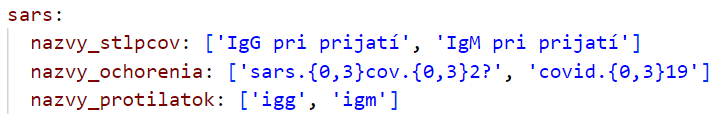
\includegraphics[width=0.85\textwidth]{images/protilatky_yaml}}
	%popis obrazku
	\caption[Ukážka zápisu testu na protilátky]{Ukážka zápisu hľadaného testu na protilátky do YAML súboru}
	%id obrazku, pomocou ktoreho sa budeme na obrazok odvolavat
	\label{obr:protilatky_yaml}
\end{figure}

\section{Spôsob modifikácie používateľom}


\section{Možnosti ďalšieho vylepšenia}

Aj napriek výraznému zlepšeniu možnosti modifikácie získavaných údajov oproti pôvodnému systému ani tento spôsob nie je dokonalý a je stále pomerne komplikovaný pre používateľa bez znalosti regulárnych výrazov a prácou s súbormi vo formáte YAML. Preto sa v tejto časti skúsime zamerať na možnosti riešenia týchto problémov. Táto časť práce je však rýdzo teoretická a samotná implementácia jednotlivých vylepšení nie je súčasťou tejto práce. 

\subsection{Určenie problémov}

Ako prvé si musíme určiť aké problémy môže mať používateľ pri práci s naším systémom. Inými slovami, čo komplikuje využívanie a modifikovanie systému. Ako bolo už v úvode tejto časti spomenuté tieto problémy sú dva a to:

\begin{itemize}
	\item používateľ musí poznať všetky časté spôsoby zápisu danej informácie a často potrebuje byť schopný písať aspoň jednoduché regulárne výrazy
	\item používateľ musí vedieť pracovať so súborom typu YAML
\end{itemize}

\subsection{Problém znalosti spôsobu zápisu informácie a regulárnych výrazov}

Podstatou tohto problému je, že vyžadujeme of používateľa hneď niekoľko znalostí ktoré nemusí mať. Konkrétne vyžadujeme aby poznal všetky časté spôsoby zápisu požadovanej informácie, napríklad chceme aby vedel že v prípade fibrilácie predsiení sa využíva aj skratka FP aj skratka FiP. Zároveň vyžadujeme aby vedel využívať syntax regulárnych výrazov, napríklad okolo skratky IM (infarkt myokardu) sa nesmú nachádzať iné písmená inak môže nastať situácia, že systém určí, že pacient na toto ochorení trpí z dôvodu, že v texte nájde meno IMRICH zapísané veľkými písmenami. 

Ďalším problémom ktorý z tohto vyplýva je nemožnosť zaručenia správnosti výsledkov keďže dané regulárne výrazy písal používateľ a preto overenie ich správneho fungovanie je na ňom. 

Ako jediné rozumné riešenie tohto problému sa javí vytvorenie databázy do ktorej by sme ručne vložili potrebné regulárne výrazy pre čo najväčšie množstvo rôznych informácii ktoré by mohol používateľ požadovať a následne dať používateľovi možnosť si vybrať ktoré z týchto informácii chce získať a dovoliť mu písať vlastné regulárne výrazy iba pre informácie ktoré nie sú obsiahnuté v databáze.

\subsection{Problém znalosti YAML formátu}

Tento problém nie je až tak závažný ako ten predchádzajúci, keďže formát YAML bol vyvíjaný tak aby bol čo najčitateľnejší pre človeka. Zároveň my nežiadame od používateľa vytváranie komplikovaných objektov ale využívanie reťazcov, zoznamov a asociatívnych polí. Avšak faktom je, že od používateľa žiadame aby modifikoval textový konfiguračný súbor čo sa dá považovať za komplikáciu.

Najrozumnejším riešením tohto problému je vytvorenie grafického používateľského rozhrania (GUI) v ktorom by používateľ mohol modifikovať množinu získavaných informácii. 